\chapter{Architecture at SAP Hybris}\label{chapter:hybris_architecture}
In this chapter, a detail research of the architecture at SAP Hybris is conducted. Firstly, the Section \ref{section:hybris_architecture/vision} clarifies vision of \acrshort{YaaS}. Secondly, the basic principles for modeling and developing microservices are listed in Section \ref{section:hybris_architecture/YaaS_architecture_principles}. In order to perceive a clear understanding about modeling and deployment process at SAP Hybris, Section \ref{section:hybris_architecture/interview} presents detailed interview conducted with various key personnels. The modeling process deduced from interviews is further clarified with an example in Section \ref{section:hybris_architecture/example_scenario}. Finally, the process of continuous deployment followed at SAP Hybris, which is one of the major processes when using microservices, is discussed in Section \ref{section:hybris_architecture/deployment_workflow}.
\section{Overview}\label{section:hybris_architecture/overview}
\acrshort{YaaS} provides a variety of business services related to different domains such as Commerce, Marketing, Billing etc. Using these offered services, the developers can create their own business services focusing more on their business requirements.\\
The Figure \ref{fig:hybris_architecture/overview/yaas_overview} provides the overview of \acrshort{YaaS}. \acrshort{YaaS} provides various business processes as a service (bPaaS) essential to develop other applications and services, thus filling up the gap between \acrshort{SaaS} and \acrshort{PaaS}.
\begin{figure}[H]
\begin{center}
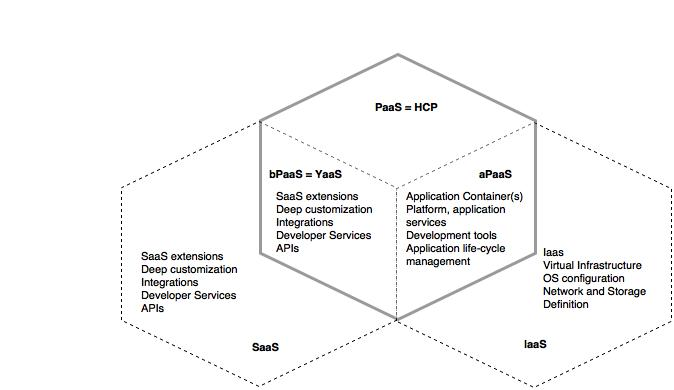
\includegraphics[width=0.6\textwidth]{figures/hybris-architecture-one}
\caption{\acrshort{YaaS} and \acrshort{HCP} \cite{Hirsch:2015aa}}
\label{fig:hybris_architecture/overview/yaas_overview}
\end{center}
\end{figure}
\\
\section{Vision}\label{section:hybris_architecture/vision}
The vision of \acrshort{YaaS} can be made clear with the following statement.
\begin{shaded}
"A cloud platform that allows everyone to easily develop, extend and sell services and applications." \\
\cite{Stubbe:2015aa}
\end{shaded}
Additionally, the vision at SAP Hybris can be broadly categorized into following objectives.\\
\begin{enumerate}
\item \textbf{Cloud First}\\
The different parts of the application need to be scaled independently.
\item \textbf{Autonomy}\\
The development teams should be able to develop their modules independent of other teams and able to freely choose the technology that fits the job.
\item \textbf{Retain Speed}\\
The new features can only be of high value to customers if could be able to be released as fast as possible.
\item \textbf{Community}\\
It should be possible for the components to be shared across internal and external developers.
\end{enumerate}
The keywords from various definitions of microservices discussed in Section \ref{tab:context/microservices_architecture_style/keywords_extracted_from_various_definitions_of_microservice} as well as the characteristics of microservices signifies clearly that microservices architecture can be a good fit for \acrshort{YaaS} architecture.
\section{SAP Hybris Architecture Principles}\label{section:hybris_architecture/YaaS_architecture_principles}
The Agile Manifesto \cite{Beck:2011aa} provides various principles to develop a software in a better way by minimizing the time for delivering new feature. It focuses on fast response to the requirement changes by continuous delivery of software artifacts with close collaboration between customer and self-organizing teams.\\
The Reactive Manifesto \cite{Boner:2014aa} lists various qualities of a reactive system which includes responsiveness (acceptable consistent response time, quick detection and solution of problem), resilience (responsive during the event of failure) , elasticity (responsive during varying amount of workload) and asynchronous message passing. Additionally, loose coupling is also highly focused.\\
Furthermore, the twelve factors from Heroku \cite{Wiggins:2012aa} provides a methodology for minimizing time and cost to develop software applications as services. It emphasizes on scalability of applications, explicit declaration as well as isolation of dependencies among the components, multiple continuous deployments from a single version controlled codebase with separate pipelines for build, release and run.\\
Finally, the microservices architectural approach provides techiques of developing an application as a collection of autonomous small sized services focused on single responsibility. [Section \ref{section:context/microservices_architecture_style}] It focuses on independent deployment capability of individual microservice and suggests to use lightweight mechanisms such as http for communication among services. The architecture offers various advantages, few of them being a) independent scalability of each microservice, b) resilience achieved by isolating failure in a component and c) technology heterogeneity among various development teams. \cite{Newman:2015aa}
\\
Following the principles mentioned above, a list of principles are compiled to be used as guidelines for creating microservices at SAP Hybris. \cite{Stubbe:2015aa}
\\
\begin{shaded}\textbf{The y-Factors}\end{shaded}
\\
\begin{enumerate}
\item \textbf{Self-Sufficient Teams}\\
The teams have freedom for any decision related to the design and development of their components. This freedom is balanced by the responsibility for the team to handle the complete lifecycle of their components including deploying, running, enhancing performance in production and troubleshooting in case of any problems.
\item \textbf{Open Technology landscape}\\
The teams are independent to choose any technology that they believe fits the requirement. They are completely responsible for the quality of their product. This gives the teams a feeling of ownership and satisfaction for their products.
\item \textbf{Release early, release often}\\
The agile manifesto and twelve factors from Heroku also focus on continuous delivery of product to the clients. This decreases time of feedback and also results in high customer satisfaction. The teams are responsible to create build and delivery pipelines for all available environments.
\item \textbf{Responsibility}\\
The teams are the only responsible groups to work directly with the customers on the behalf of their products. They need to work on the feedbacks provided by the customers. It increases the quality of the products and relationship with customers. All the responsibilities including scaling, maintaining, supporting and improving products are handled by the respective teams.
\item \textbf{\acrshort{API}s first}\\
\acrshort{API} is a contract between the service and the consumers. The decision regarding design and development of \acrshort{API} is very crucial. \acrshort{API} can be one of the greatest assets if good or else can be a huge liability. \cite{Bloch:2016aa} The articles \cite{Bloch:2016aa} and \cite{Blanchette:2008aa} list various characteristics of good \acrshort{API} including a) simplicity, b) extensibility, c) maintainability, d) completeness, e) small and f) focussing on single functionality. Furthermore, a good approach to develop \acrshort{API} is to first design iteratively before implementation in order to understand the requirement clearly. Another important aspect of a good \acrshort{API} is a complete and updated documentation.
\item \textbf{Predictable and easy-to-use UI}\\
The user interfaces should be simple, consistent across the system and also comply with various user friendly patterns.\cite{Sollenberger:2012aa} The articles \cite{Martin:2013aa} and \cite{Porter:2016aa} specify additional principles to be considered when designing user interfaces. A few of them are a) providing clarity with regard to purpose, b) smart organization and c) respecting the expectation as well as requirements of customers.
\item \textbf{Small and Simple Services}
A service should be small and focused on cohesive functionalities. The concept closely relates to the single responsibility principle. \cite{Martin:2016aa} A good approach is to explicitly create boundaries around business capabilities.\cite{Newman:2015aa}
\item \textbf{Scalability of technology}\\
The choice of technologies should be cloud friendly such that the products can scale cost-efficiently and without any delay. It is influenced by the elasticity principle provided by the reactive manifesto.\cite{Boner:2014aa}
\item \textbf{Design for failure}
The service should be responsive at the time of failure. It can be possible by the containment and the isolation of failure within each component. Similarly, the recovery should be handled gracefully without affecting the overall availability of the entire system. \cite{Boner:2014aa}
\item \textbf{Independent Services}\\
The services should be autonomous. Each service should be able to be deployed independently. The services should be loosely coupled, they could be changed independently of eachother. The concept is highly enforced by exposing functionalities via \acrshort{API}s and using lightweight network calls as only way of communication among services. \cite{Newman:2015aa}
\item \textbf{Understand Your System}\\
It is crucial to have a good understanding of problem domain in order to create a good design. The concept of domain driven design strongly supports this approach and motivates to indentify individual autonomous components, their boundaries and the communication patterns among them. \cite{Newman:2015aa} Furthermore, it is also important to understand the expectations of the consumers regarding performance and then to realize them accordingly. However, this can only be possible by installing necessary operational capabilities such as a) continuous delivery, b) monitoring, c) scaling and d) resilience.
\end{enumerate}
 \section{Modeling Microservices at SAP Hybris}\label{section:hybris_architecture/interview}
 With the intension to anticipate the overall belief, culture and practice followed by SAP Hybris for developing \acrshort{YaaS}, a number of interviews are conducted with a subset of key personnels who are directly involved in \acrshort{YaaS} at different roles. The list of interviewees with their corresponsing roles is shown in the Table \ref{tab:hybris_architecture/interview/interviewee_list}. In order to preserve identity, the real names are replaced with forged ones.
\begin{table}[H]
  \centering
  \begin{adjustbox}{max width=\textwidth}
  \begin{tabular}{*{14}{|c}|}%%{|c|l|}
  \hline
\textbf{Names}          & \textbf{Roles}\\      \hline
John Doe                & Product Manager\\     \hline
Ivan Horvat             & Senior Developer\\    \hline
Jane Doe                & Product Manager\\     \hline
Mario Rossi             & Product Manager\\     \hline
Nanashi No Gombe        & Product Manager\\     \hline
Hans Meier              & Architect\\           \hline
Otto Normalverbraucher  & Product Manager\\     \hline
Jan Kowalski            & Senior Developer\\    \hline
\end{tabular}
\end{adjustbox}
  \caption{Interviewee List}
  \label{tab:hybris_architecture/interview/interviewee_list}
\end{table}
\\
\subsection{Hypothesis}\label{section:hybris_architecture/interview/hypothesis}
During the process of solving the concerned research questions, various topics of high value have been discovered. The topics are:\\
\begin{enumerate}
\item Granularity
\item Quality Attributes
\item Process to design microservices
\end{enumerate}
\\
Similarly, based on research findings, a list of hypothesis has been built for each topic listed in the list above.

\begin{shaded}
Hypothesis 1:
\end{shaded}\label{section:hybris_architecture/interview/hypothesis_1}
\textbf{The correct size of microservices is determined by: \begin{enumerate}\item Single Responsibility Principle \item Autonomy, and \item Infrastructure Capability \end{enumerate}}
\\
According S.Newman, a good microservice should be small and should focus on accomplishing one thing well. Additionally, it could be independently deployed and updated. This strongly suggests the requirement of \acrshort{SRP} and autonomy respectively. \cite{Newman:2015aa} Futhermore, M. Stine also agrees that the size of a microservice should be determined by single responsibility principle \cite{Stine:2014aa}. \\
Also, the principle mentioned in \ref{principle:granularity/IT_infrastructure} indicates that the advancement in the current technology and culture of the organization influences the size of the microservices. \cite{Pierre-Reldin:2007aa}
\begin{shaded}
Hypothesis 2:
\end{shaded} \label{section:hybris_architecture/interview/hypothesis_2}
\textbf{Domain driven design is the optimum approach to design microservices.}
\\
\\
The concept of domain driven design to design the microservices is suggested by S. Newman and M. Fowler \cite{Newman:2015aa} \cite{Fowler:2014aa}. Similary, there can be found evidence of domain driven design being used in various projects to design microservices. The list of projects is shown in the Table \ref{tab:domain_driven_design/microservices_and_bounded_context/Microservices_following_Bounded_Context}.
\\
\subsection{Interview Compilation}\label{section:hybris_architecture/interview/interview_compilation}
For each of the topics listed in Section \ref{section:hybris_architecture/interview/hypothesis}, a list of questionaires is prepared. The questions are asked to the interviewees. In the remaining part of this section, the responses from the interviews on the questionaires are compiled.
\\
\textbf{\underline{1. Granularity}}\\  
\begin{shaded} Question 1.1 \end{shaded} \label{question:hybris_architecture/interview/question_1.1}
"Do you consider the size of microservices when desigining microservices architecture?"\\
\begin{comment}
\begin{table}[H]
\centering
\begin{adjustbox}{max width=\textwidth}
\begin{tabular}{*{14}{|c}|}%%{|c|l|l|l|l|l|l|l|l|l|}
\hline
\textbf{Response 1.1} & John & Ivan & Jane & Mario & Nanashi & Hans & Otto & Jan & \textbf{Score}\\
 \hline
Important               & 1 & 1 & 1 & 0 & 1 & 1 & 0 & 0 & \textbf{5}    \\ 
 \hline
Secondary, Not primary  & 0 & 0 & 0 & 1 & 0 & 0 & 1 & 1 & \textbf{3} \\ 
 \hline
Not Important           & 0 & 0 & 0 & 0 & 0 & 0 & 0 & 0 & \textbf{0} \\ 
 \hline
 \hline
\end{tabular}
\end{adjustbox}
\label{tab:hybris_architecture/interview/question_1.1}
\end{table}
\end{comment}
\begin{comment}
\begin{figure}[H]
\begin{center}
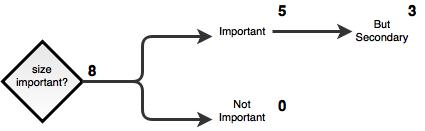
\includegraphics[width=0.5\textwidth]{figures/hybris_architecture_question_1_1}
\label{fig:hybris_architecture/interview/hybris-architecture-question-1-1}
\end{center}
\end{figure}
\\
\end{comment}

\begin{figure}[H]
\begin{center}
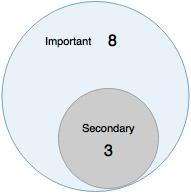
\includegraphics[scale=0.5]{figures/question1_1}
\label{fig:hybris_architecture/interview/question1-1}
\end{center}
\end{figure}
\\

\begin{shaded} Question 1.2 \end{shaded} \label{question:hybris_architecture/interview/question_1.2}
"How do you measure size of a microservice?"\\
\begin{comment}
\begin{table}[H]
\centering
\begin{adjustbox}{max width=\textwidth}
\begin{tabular}{*{14}{|c}|}%%{|c|c|l|l|l|l|l|l|l|l|l|}
\hline
\multicolumn{2}{|c|}{\textbf{Response 1.2} }& John & Ivan & Jane & Mario & Nanashi & Hans & Otto & Jan & \textbf{Score}\\
 \hline
 \hline
\multicolumn{2}{|c|}{\textit{Qualitatively}}               & 1 & 1 & 1 & 1 & 1 & 1 & 1 & 1 & \textbf{8}    \\ 
 \hline
a.& Functionality  & 1 & 1 & 1 & 1 & 1 & 1 & 1 & 1 & \textbf{8}\\ 
 \hline
b.& Business value           & 1 & 1 & 1 & 1 & 1 & 1 & 1 & 1 & \textbf{8} \\ 
 \hline
 \hline
 \multicolumn{2}{|c|}{\textit{Quantitatively}}               & 0 & 0 & 0 & 0 & 0 & 0 & 0 & 0 & \textbf{0}    \\ 
 \hline
 \hline
\end{tabular}
\end{adjustbox}
\label{tab:hybris_architecture/interview/question_1.2}
\end{table}
\end{comment}
\\
\begin{comment}
\\
\begin{figure}[H]
\begin{center}
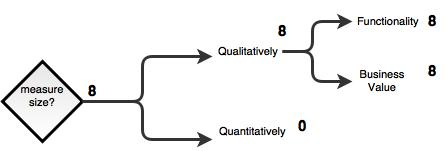
\includegraphics[width=0.9\textwidth]{figures/hybris_architecture_question_1_2}
\label{fig:hybris_architecture/interview/hybris-architecture-question-1-2}
\end{center}
\end{figure}
\\
\end{comment}

\\
\begin{figure}[H]
\begin{center}
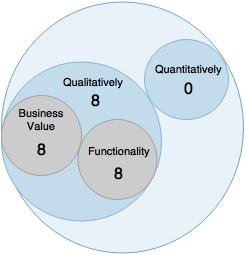
\includegraphics[scale=0.5]{figures/question1_2}
\label{fig:hybris_architecture/interview/question1-2}
\end{center}
\end{figure}
\\

\begin{shaded} Question 1.3 \end{shaded} \label{question:hybris_architecture/interview/question_1.3}
"What factors do you consider when you decide the size of a microservice?"\\

\begin{comment}
\begin{table}[H]
\centering
\begin{adjustbox}{max width=\textwidth}
\begin{tabular}{*{14}{|c}|}%%{|c|c|l|l|l|l|l|l|l|l|l|}
\hline
\multicolumn{2}{|c|}{\textbf{Response 1.3} }
                                    & John & Ivan & Jane & Mario & Nanashi & Hans & Otto & Jan & \textbf{Score}\\
 \hline
 \hline
\multicolumn{2}{|c|}{\textit{as small as possible in terms of functionality}}               
                                    & 1 & 1 & 1 & 1 & 1 & 1 & 1 & 1 & \textbf{8}    \\ 
 \hline
 \hline
 \multicolumn{2}{|c|}{\textit{influenced by other attributes}}               
                                    &   &   &   &   &   &   &   &   &     \\ 
 \hline
a.& Business Value                  & 1 & 1 & 1 & 1 & 1 & 1 & 1 & 1 & \textbf{8}\\ 
 \hline
b.& Single Responsibility           & 1 & 1 & 1 & 1 & 1 & 1 & 1 & 1 & \textbf{8} \\ 
 \hline
c.& Loose Coupling                  & 0 & 1 & 0 & 0 & 1 & 1 & 0 & 1 & \textbf{4} \\ 
 \hline
d.& Cohesion                        & 0 & 1 & 0 & 0 & 0 & 0 & 1 & 1 & \textbf{3} \\ 
 \hline
e.& Autonomy                        & 0 & 1 & 1 & 0 & 0 & 1 & 0 & 0 & \textbf{3} \\ 
 \hline
f.& Maintainability                 & 0 & 1 & 0 & 0 & 0 & 1 & 1 & 0 & \textbf{3} \\ 
 \hline
g.& Reusability                     & 0 & 1 & 0 & 0 & 1 & 1 & 1 & 0 & \textbf{4} \\ 
 \hline
h.& Scalability                     & 1 & 1 & 0 & 1 & 1 & 1 & 1 & 0 & \textbf{6} \\ 
 \hline
i.& Network Complexity              & 1 & 0 & 0 & 0 & 1 & 1 & 0 & 0 & \textbf{3} \\ 
 \hline
 \hline
\end{tabular}
\end{adjustbox}
\label{tab:hybris_architecture/interview/question_1.3}
\end{table}
\end{comment}
\\
\begin{comment}
\\
\begin{figure}[H]
\begin{center}
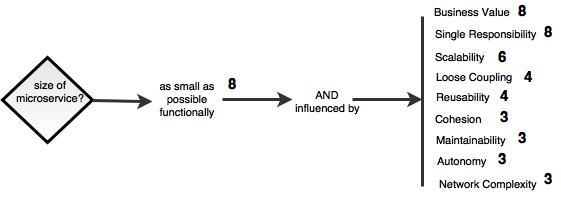
\includegraphics[width=0.9\textwidth]{figures/hybris_architecture_question_1_3}
\label{fig:hybris_architecture/interview/hybris-architecture-question-1-3}
\end{center}
\end{figure}
\\
\end{comment}
\\
\begin{figure}[H]
\begin{center}
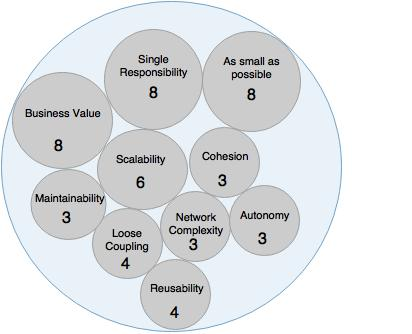
\includegraphics[scale=0.5]{figures/question1_3}
\label{fig:hybris_architecture/interview/question1-3}
\end{center}
\end{figure}
\\
\begin{shaded} Question 1.4 \end{shaded} \label{question:hybris_architecture/interview/question_1.4}
"Suppose that you do not have the agile culture like continuous integration and delivery automation and also cloud infrastructure. How will it affect your decision regarding microservices and their size?"\\
\begin{table}[H]
\centering
\begin{adjustbox}{max width=\textwidth}
\begin{tabular}{*{14}{|c}|}%%{|c|l|l|l|l|l|l|l|l|l|}
\hline
\textbf{Response 1.4}   & John & Ivan & Jane & Mario & Nanashi & Hans & Otto & Jan & \textbf{Score}\\
 \hline
 \begin{tabular}{ll}
                    \multirow{2}{*}
                    & No microservices at all, start with Monolith,\\
                    & extract one microservice at a time as automation matures\\
                    \end{tabular}
               
                                & 1 & 1 & 0 & 1 & 1 & 1 & 1 & 1 & \textbf{7}    \\ 
 \hline
  \begin{tabular}{ll}
                    \multirow{2}{*}
                    & Start with bigger sized microservices with\\
                    & high business value, low coupling and single Responsibility\\
                    \end{tabular}  
                                & 0 & 0 & 1 & 0 & 1 & 0 & 1 & 0 & \textbf{3} \\ 
 \hline
 \hline
\end{tabular}
\end{adjustbox}
\label{tab:hybris_architecture/interview/question_1.4}
\end{table}
\\
\begin{comment}
\\
\begin{figure}[H]
\begin{center}
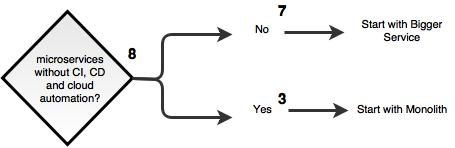
\includegraphics[width=0.9\textwidth]{figures/hybris_architecture_question_1_4}
\label{fig:hybris_architecture/interview/hybris-architecture-question-1-4}
\end{center}
\end{figure}
\\
\\
\begin{figure}[H]
\begin{center}
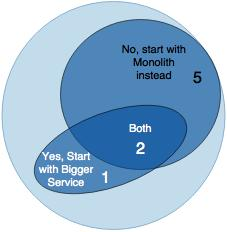
\includegraphics[scale=0.5]{figures/question1_4}
\label{fig:hybris_architecture/interview/question1-4}
\end{center}
\end{figure}
\\
\end{comment}
\begin{shaded} Question 1.5 \end{shaded} \label{question:hybris_architecture/interview/question_1.5}
"Are you facing any complexities because of microservices architecture and the size you have chosen?"\\
\begin{table}[H]
\centering
\begin{adjustbox}{max width=\textwidth}
\begin{tabular}{*{14}{|c}|}%%{|c|l|l|l|l|l|l|l|l|l|}
\hline
\textbf{Response 1.5}   & John & Ivan & Jane & Mario & Nanashi & Hans & Otto & Jan & \textbf{Score}\\
 \hline
communication overhead in network               & 0 & 1 & 0 & 0 & 0 & 0 & 1 & 0 & \textbf{2}    \\ 
 \hline
complexity in failure handling  & 0 & 1 & 0 & 0 & 0 & 0 & 0 & 0 & \textbf{1} \\ 
 \hline
Monitoring is difficult           & 0 & 1 & 0 & 0 & 0 & 0 & 1 & 0 & \textbf{1} \\ 
 \hline
 Operational support is costly           & 0 & 1 & 1 & 0 & 0 & 0 & 0 & 0 & \textbf{2} \\ 
 \hline
 difficult to trace a request           & 0 & 1 & 1 & 0 & 0 & 0 & 0 & 0 & \textbf{2} \\ 
 \hline
 updates can be difficult due to dependencies among microservices          & 0 & 0 & 1 & 0 & 0 & 0 & 0 & 0 & \textbf{1} \\ 
 \hline
 \hline
\end{tabular}
\end{adjustbox}
\label{tab:hybris_architecture/interview/question_1.5}
\end{table}
\\


\textbf{\underline{2. Quality Attributes}}\\
\begin{shaded} Question 2.1 \end{shaded} \label{question:hybris_architecture/interview/question_2.1}
"Do you consider any quality attributes when selecting microservices?"\\
\begin{table}[H]
\centering
\begin{adjustbox}{max width=\textwidth}
\begin{tabular}{*{14}{|c}|}%%{|c|l|l|l|l|l|l|l|l|l|}
\hline
\textbf{Response 2.1}   & John & Ivan & Jane & Mario & Nanashi & Hans & Otto & Jan & \textbf{Score}\\
 \hline
Loose Coupling          & 1 & 1 & 1 & 1 & 1 & 1 & 1 & 1 & \textbf{8}    \\ 
 \hline
Cohesion                & 1 & 1 & 1 & 1 & 1 & 1 & 0 & 1 & \textbf{7}    \\ 
 \hline
 Autonomy               & 1 & 1 & 0 & 0 & 0 & 1 & 1 & 0 & \textbf{4}    \\ 
 \hline
 Scalability            & 1 & 0 & 0 & 1 & 1 & 0 & 1 & 1 & \textbf{5}    \\ 
 \hline
 Complexity             & 1 & 0 & 0 & 0 & 1 & 0 & 1 & 0 & \textbf{3}    \\ 
 \hline
 Reusability            & 0 & 1 & 0 & 0 & 0 & 0 & 1 & 0 & \textbf{2}    \\ 
 \hline
 \hline
\end{tabular}
\end{adjustbox}
\caption{Response 2.1}
\label{tab:hybris_architecture/interview/question_two_one}
\end{table}
\\

\begin{shaded} Question 2.2 \end{shaded} \label{question:hybris_architecture/interview/question_2.2}
"Do you consider any metrics for evaluating the quality attributes?"
\begin{comment}
\begin{table}[H]
\centering
\begin{adjustbox}{max width=\textwidth}
\begin{tabular}{*{14}{|c}|}%%{|c|l|l|l|l|l|l|l|l|l|}
\hline
\textbf{Response 2.2}   & John & Ivan & Jane & Mario & Nanashi & Hans & Otto & Jan & \textbf{Score}\\
 \hline
No          & 1 & 1 & 1 & 1 & 1 & 1 & 1 & 1 & \textbf{8}    \\ 
 \hline
Yes                & 0 & 0 & 0 & 0 & 0 & 0 & 0 & 0 & \textbf{0}    \\ 
 \hline
\end{tabular}
\end{adjustbox}
\label{tab:hybris_architecture/interview/question_2.2}
\end{table}
\end{comment}
\begin{comment}
\\
\begin{figure}[H]
\begin{center}
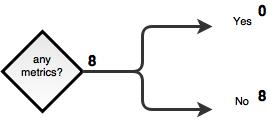
\includegraphics[scale=0.5]{figures/hybris_architecture_question_2_2}
\label{fig:hybris_architecture/interview/hybris-architecture-question-2-2}
\end{center}
\end{figure}
\end{comment}
\begin{figure}[H]
\begin{center}
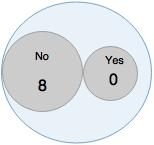
\includegraphics[scale=0.5]{figures/question2_2}
\label{fig:hybris_architecture/interview/question2-2}
\end{center}
\end{figure}
\begin{shaded} Question 2.3 \end{shaded} \label{question:hybris_architecture/interview/question_2.3}
"Do you think the table of basic metrics can be helpful?"
\begin{comment}
\begin{table}[H]
\centering
\begin{adjustbox}{max width=\textwidth}
\begin{tabular}{*{14}{|c}|}%%{|c|l|l|l|l|l|l|l|l|l|}
\hline
\textbf{Response 2.3}   & John & Ivan & Jane & Mario & Nanashi & Hans & Otto & Jan & \textbf{Score}\\
 \hline
No          & 0 & 0 & 0 & 0 & 0 & 0 & 0 & 0 & \textbf{0}    \\ 
 \hline
Yes                & 1 & 0 & 1 & 0 & 1 & 0 & 1 & 0 & \textbf{4}    \\ 
 \hline
Maybe                & 0 & 1 & 0 & 1 & 0 & 1 & 0 & 1 & \textbf{4}    \\ 
 \hline
 \hline
\end{tabular}
\end{adjustbox}
\label{tab:hybris_architecture/interview/question_2.3}
\end{table}
\end{comment}
\begin{comment}
\begin{figure}[H]
\begin{center}
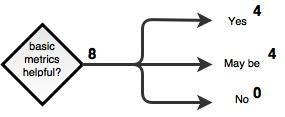
\includegraphics[scale=0.5]{figures/hybris_architecture_question_2_3}
\label{fig:hybris_architecture/interview/hybris-architecture-question-2-3}
\end{center}
\end{figure}
\end{comment}

\begin{figure}[H]
\begin{center}
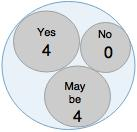
\includegraphics[scale=0.5]{figures/question2_3}
\label{fig:hybris_architecture/interview/question2-3}
\end{center}
\end{figure}
\\
\textbf{\underline{3. Process to design microservices}}\\
\begin{shaded} Question 3.1 \end{shaded} \label{question:hybris_architecture/interview/question_3.1}
"Do you follow specific set of consistent procedures across the teams to discover microservices?"
\begin{comment}
\begin{table}[H]
\centering
\begin{adjustbox}{max width=\textwidth}
\begin{tabular}{*{14}{|c}|}%%{|c|l|l|l|l|l|l|l|l|l|}
\hline
\textbf{Response 3.1}   & John & Ivan & Jane & Mario & Nanashi & Hans & Otto & Jan & \textbf{Score}\\
 \hline
No          & 1 & 1 & 1 & 1 & 1 & 1 & 1 & 1 & \textbf{8}    \\ 
 \hline
Yes                & 0 & 0 & 0 & 0 & 0 & 0 & 0 & 0 & \textbf{0}    \\ 
 \hline
\end{tabular}
\end{adjustbox}
\label{tab:hybris_architecture/interview/question_2.3}
\end{table}
\end{comment}
\begin{comment}
\\
\begin{figure}[H]
\begin{center}
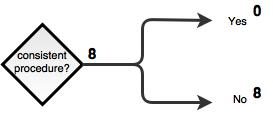
\includegraphics[scale=0.5]{figures/hybris_architecture_question_3_1}
\label{fig:hybris_architecture/interview/hybris-architecture-question-3-1}
\end{center}
\end{figure}
\\
\end{comment}
\begin{figure}[H]
\begin{center}
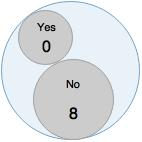
\includegraphics[scale=0.5]{figures/question3_1}
\label{fig:hybris_architecture/interview/question3-1}
\end{center}
\end{figure}
\\
\begin{shaded} Question 3.2 \end{shaded} \label{question:hybris_architecture/interview/question_3.2}
"Can you define the process you follow to come up with microservices?"
\begin{comment}
\begin{table}[H]
\centering
\begin{adjustbox}{max width=\textwidth}
\begin{tabular}{*{14}{|c}|}%%{|c|l|l|l|l|l|l|l|l|l|l|}
\hline
\multicolumn{3}{|c|}{\textbf{Response 3.2}}   & John & Ivan & Jane & Mario & Nanashi & Hans & Otto & Jan & \textbf{Score}\\
\hline
\hline
\multicolumn{3}{|c|}{
\begin{tabular}{ll}
\multirow{4}{*}
& By brain-storming to divide a usecase into finer\\
& functionalities considering business value, cohesion,\\
& loose coupling [Single Responsibility], autonomy,\\
& reusability and scalability.
\end{tabular}}
                                            & 1 & 0 & 1 & 1 & 0 & 0 & 1 & 1 & \textbf{5}    \\ 
 \hline
& \multicolumn{2}{|c|}{\textit{Have you heard of Domain driven design and bounded context?}}               
                                            &   &   &   &   &   &   &   &   &      \\ 
 \hline
 & & Yes                                    & 0 &   & 0 & 0 &   &   & 1 & 0 & \textbf{1}    \\ 
 \hline
 & \multicolumn{2}{|c|}{\textit{Is the concept provided by bounded context being used?}}               
                                            &   &   &   &   &   &   &   &   &      \\ 
 \hline
 & & Yes                                    & 1 & 0 & 1 & 0 & 0 & 0 & 1 & 0 & \textbf{3}    \\
 \hline
 \hline
\multicolumn{3}{|c|}{
\begin{tabular}{ll}
\multirow{4}{*}
& By identifying bounded context using domain-driven-design\\
& Understand the problem domain interacting with\\
& domain experts and studying the interaction among\\
& domain models and flow of data.
\end{tabular}}
                                            & 0 & 1 & 0 & 0 & 1 & 1 & 1 & 0 & \textbf{4}    \\ 
\hline
\hline
\end{tabular}
\end{adjustbox}
\label{tab:hybris_architecture/interview/question_3.2}
\end{table}
\end{comment}
\begin{comment}
\\
\begin{figure}[H]
\begin{center}
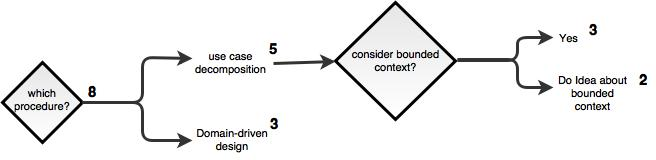
\includegraphics[scale=0.5]{figures/hybris_architecture_question_3_2}
\label{fig:hybris_architecture/interview/hybris-architecture-question-3-2}
\end{center}
\end{figure}
\end{comment}
\begin{figure}[H]
\begin{center}
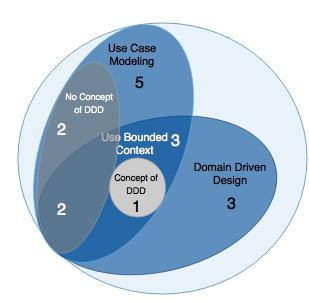
\includegraphics[scale=0.5]{figures/question3_2}
\label{fig:hybris_architecture/interview/question3-2}
\end{center}
\end{figure}
\\
\subsection{Interview Reflection on Hypothesis}\label{section:hybris_architecture/interview/interview_reflection_on_hypothesis}
The data gathered from the interviews which are compiled in the Section \ref{section:hybris_architecture/interview/interview_compilation} can be a good source to analyze the hypothesis listed on the Section \ref{section:hybris_architecture/interview/hypothesis}.
\\
\begin{shaded} Hypothesis 1 \end{shaded}
\textbf{The correct size of microservices is determined by: \begin{enumerate}\item Single Responsibility Principle \item Autonomy, and \item Infrastructure Capability \end{enumerate}}
\\
The response from Question 1.3 [\ref{question:hybris_architecture/interview/question_1.3}] has helped to point out some important constraints which play significant role in industries while choosing appropriate size of the microservices. It can be deduced that the answer closely relate to the Hypothesis \ref{section:hybris_architecture/interview/hypothesis_1}. The Figure \ref{fig:hybris_architecture/interview/attributes_grouping} attempts to clarify the relationship among the terms with the hypothesis.
\\

\\
\begin{figure}[H]
\begin{center}
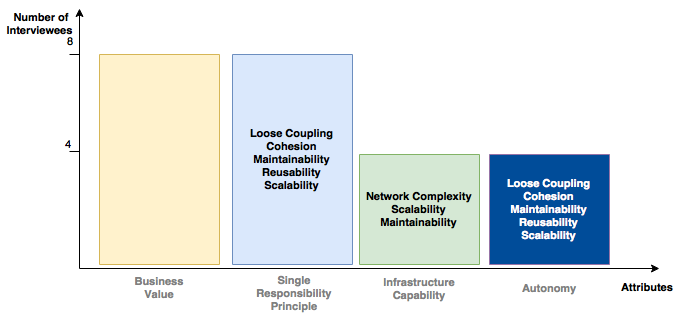
\includegraphics[width=0.8\textwidth]{figures/hybris-architecture-two}
\caption{Attributes grouping from interview response}
\label{fig:hybris_architecture/interview/attributes_grouping}
\end{center}
\end{figure}
\\
The interview unfolds various quality attributes affecting the correct size of a microservice. Moreover, these quality attributes can be arranged into three major groups, which are: \\
\begin{enumerate}
\item Single Responsibility Principle
\item Automony
\item Infrastructure Capability
\end{enumerate}
\\
The response from the Question 1.4 [\ref{question:hybris_architecture/interview/question_1.4}] highly suggests the significance of proper infrastructure to determine the size of the microservices and also regarding the choice of using microservices architecture.
This highly moves in the direction to support the hypothesis.\\
Finally, there appears one additional constraint to affect the size of the microservices, which is not covered by hypothesis but mentioned by all interviewees, the \textbf{business value} provided by the microservices.
\\
\begin{shaded} Hypothesis 2 \end{shaded}
\textbf{Domain driven design is the optimum approach to design microservices.}
\\
From the response to Question 3.1 [\ref{question:hybris_architecture/interview/question_3.1}], it can be implied that the organization has no consistent set of specific guidelines which are agreed and pratised across all teams. However,  
the various reactions to the Question 3.2 [\ref{question:hybris_architecture/interview/question_3.2}] suggest that the process fall under two classes. The representation of response from \ref{question:hybris_architecture/interview/question_3.2} is repeated here again for convenience \ref{fig:hybris_architecture/interview/process_variations_to_design_microservices}.\\
\\
\begin{figure}[H]
\begin{center}
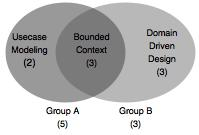
\includegraphics[scale=0.5]{figures/hybris-architecture-three}
\caption{Process variations to design microservices}
\label{fig:hybris_architecture/interview/process_variations_to_design_microservices}
\end{center}
\end{figure}
\\
According to one category of reaction, some teams functionally divide a usecase into small functions based upon various factors such as single responsiblity and the requirements of performance. This strongly resembles to the use cases modeling technique as described in the Chapter \ref{section:selection_by_use_case/use_case}. 
\\Moreover, within the same group, a partition of teams are also using the concept of bounded context to ensure autonomy, which also suggests towards the direction of domain driven design approach as mentioned in the Chapter \ref{section:domain_driven_design/introduction}. It is interesting to find out that some of the teams are using the concept of bounded context implicitly even without its knowledge. The rest of the teams who are not using bounded context, have no idea about the concept. It can be implied that they may have different view once they get familiar with the concept.
\\
Finally, the rest of the interviewees agree on domain driven design approach to be the process of designing microservices. So, the  response is of mixed nature, both use cases modeling approach and domain driven design approach are used in desigining microservices. However, it should also be stated that domain driven design are used on its own or along with usecase modeling to design the autonomous microservices.

 \section{Modeling Approach at SAP Hybris derived by interview compilation}\label{section:hybris_architecture/interview_summary}
 The responses from the interviews as compiled in Section \ref{section:hybris_architecture/interview/interview_compilation} are analyzed for each topic listed in \ref{section:hybris_architecture/interview/hypothesis} separately.
 \\
 \\
 \textbf{Granularity}
 \\
 \\
Granularity of a microservice is considered as an important aspect when implementing microservices architecture. The first impression in major cases is to make the size of microservice as small as possible. However there are also various attributes and concepts which affects the decision regarding the size of the microservices. The major aspects are single responsibility principle, autonomy and infrastructure capability.
\\
The single responsibility influences to make the size of a microservice as small as possible so that the microservice has minimum cohesive functionality and less number of consumers. On the other hand, in order to make the microservice autonomous, the microservice should have full control over its resources and have less dependencies upon other microservices for accomplishing its core logic. This suggests that the size of the microservice should be big enough to cover the transactional boundary required for its core logic and have full control on its business resources.
\\
Moreover, the small the size of the service is, the number of required microservices increases for accomplishing the functionalities of the application. This increases network complexity. Additionally, the logical complexity as well as maintainability also increase. Undoubtedly, the independent scalability of individual microservice also increases. However, this increases the operational complexity for maintaining and deploying the microservices due to the increased number of microservices.
\\
As shown in Figure \ref{fig:hybris_architecture/interview/attributes_grouping}, various factors affect the size of microservices.
The research findings as well as interview response leads to the idea that the question regarding "size" of a microservices has no straight answer. The answer itself is a multiple objective optimization problem and depends upon a) the level of abstraction of the problem domain, b) self-governance requirement, c) self-containment requirement and d) the honest capability of the organization to handle the operational complexity.
\\
Finally, there is an additional deciding factor called "Business Value". The chosen size of the microservice should provide business value and competitive advantage to the organization and closely lean towards the organizational goals. A decision for a group of cohesive functionalities to be assigned as a single microservice means that a dedicated amount of resources in terms of development, scaling, maintainance, deployment and cloud infrastructure have to be assigned. A rational decision can be to evaluate the expected business value of the microservice against the expected cost value required by it.
\\
\\
\textbf{Quality Attributes}
\\
\\
The teams do not follow any quantitative metrics for measuring various quality attributes. However, they agree on a common list of quality attributes to be considered as shown in the Table \ref{tab:hybris_architecture/interview/question_two_one} . According to the reactions from interviews, the basic metrics to evaluate the quality attributes visualized in the Table  \ref{tab:quality_of_service/quality_attributes/basic_quality_metrics} can be helpful to model microservices architecture in an efficient way.
\\
\\
\textbf{Process to design microservices}
\\
\\
There is no single consistent process followed across all the teams at SAP Hybris. Each team has its own steps to come up with microservices. However, the steps and decision are highly influenced by a set of \abrshort{YaaS} standard principles \ref{section:hybris_architecture/YaaS_architecture_principles} and vision of SAP Hybris \ref{section:hybris_architecture/vision}. The reactions from the interviewees are already visualized in \ref{fig:hybris_architecture/interview/process_variations_to_design_microservices}. 
\\
The process followed by a portion of teams closely relate to usecase modeling approach, where a usecase is divided into several smaller abstractions guided by a) cohesion, b) reusability and c) single responsibility principle. Within this group, a major number of teams also use the concept of bounded context in order to realize autonomous boundary around the microservices. Finally, the remaining portion of the teams closely follow domain driven design approach, where a problem domain is divided into sub-domains. In each sub-domain, various bounded contexts are discovered, which is then mapped into microservices. 
\\
The domain driven design approach can be considerd as the most suitable technique to design microservices. Following this approach, not only the problem domain is functionally divided into cohesive group of functionalities but also leads to a natural boundary around the cohesive functionalities closely relating to the real world scenario of the organization. Moreover, following the domain driven design approach, similarities as well as differences in concepts are acknowledged. Finally, the ownership of business resources and core logic are well preserved.

 \section{Case Study}\label{section:hybris_architecture/example_scenario}
 \acrshort{YaaS} provides a cloud platform where the customers can buy and sell applications and services related to the commerce domain. In order to accomplish this, \acrshort{YaaS} offers various basic business and core functionalities as microservices. The customers can either use or extend these services and create new services and applications focusing on their individual requirements and goals.
 \\
The following part of this section discuss the steps used to identify microservices under commerce domain in \acrshort{YaaS}.
\\
\textbf{\underline{Step 1:}}
\\
The problem domain is studied thoroughly to identify core domains, supporting domains and generic domains.
\begin{table}[H]
  \centering
  \begin{adjustbox}{max width=\textwidth}
  \begin{tabular}{*{14}{|c}|}%%{|c|c|c|}
  \hline
  \# & \textbf{Sub-domain}  & \textbf{Type} & \textbf{Description}\\
  \hline
  \hline
   1 & Checkout             & Core          & handles overall process from cart creation to selling of cart items.\\ \hline \hline
   2 & Product              & Supporting    & deals with product inventory\\ \hline
   3 & Customer             & Supporting    & deals with customer inventory\\ \hline
   4 & Coupon               & Supporting    & deals with coupon management \\ \hline
   5 & Order                & Supporting    & handles orders management\\ \hline
   6 & Site                 & Supporting    & handles site configuration\\ \hline
   7 & Tax                  & Supporting    & handles tax configuration and tax calculation\\ \hline
   8 & Payment              & Supporting    & handles payment for orders\\ \hline \hline
   9 & Email                & Generic       & provides REST api for sending emails\\ \hline
   10 & Pubsub              & Generic       & provides asynchronous event based notification service\\ \hline
   11 & Account             & Generic       & handles users and roles management\\ \hline
   12 & OAuth2              & Generic       & provides authentication for clients to access resource of resource-owner \\ \hline
   13 & Schema              & Generic       & storing schema of documents \\ \hline
   14 & Document            & Generic       & provides storage apis for storing and accessing documents \\
   \hline 
   \hline
   \end{tabular}
\end{adjustbox}
  \caption{Sub-domains in \acrshort{YaaS}}
  \label{tab:hybris_architecture/example_scenario/sub-domains-in-YaaS}
\end{table}
\\
\textbf{\underline{Step 2:}}
\\
The major functionality of the commerce platform is to sell products, which makes 'Checkout' the core sub-domain. The sub-domain is also responsible for a bunch of other independent functionalities such as cart management and cart calculation. These individual independent functionalities can be rightfully represented by bounded contexts as shown in the Table \ref{tab:hybris_architecture/example_scenario/bounded-context-in-Checkout}. The bounded contexts are realized using microservices. The other major reason for them to be made microservices, in addition to single independent responsibility, is different scalability requirements for each functionality.
\begin{table}[H]
  \centering
  \begin{adjustbox}{max width=\textwidth}
  \begin{tabular}{*{14}{|c}|}%%{|c|c|}
  \hline
  \# & \textbf{Bounded Context}  & \textbf{Description}\\
  \hline
  \hline
   1 & Checkout             & handles the orchestration logic for checkout \\ \hline
   2 & Cart                 & handles cart inventory \\ \hline
   3 & Cart Calculation     & calculates net value of cart considering various constraints such as tax, discount etc. 
   \\ \hline
   \hline
   \end{tabular}
\end{adjustbox}
  \caption{Bounded Contexts in Checkout}
  \label{tab:hybris_architecture/example_scenario/bounded-context-in-Checkout}
\end{table}
\\
\textbf{\underline{Step 3:}}
\\
The supporting sub-domain "Product" deals with various functionalities related to "Product".
\begin{table}[H]
  \centering
  \begin{adjustbox}{max width=\textwidth}
  \begin{tabular}{*{14}{|c}|}%%{|c|c|}
  \hline
  \# & \textbf{Bounded Context}  & \textbf{Description}\\
  \hline
  \hline
   1 & Category     & manage category of products \\ \hline
   2 & Product      & manage product inventory\\ \hline
   3 & Price        & manage price for products \\ \hline
   \hline
   \end{tabular}
\end{adjustbox}
  \caption{Functional Bounded Contexts in Product}
  \label{tab:hybris_architecture/example_scenario/functional-bounded-contexts-in-Product}
\end{table}
\\
The bounded contexts listed in Table \ref{tab:hybris_architecture/example_scenario/functional-bounded-contexts-in-Product} are based upon the independent responsibility and different performance requirement. Although, each functionality deals with business entity "Product", the conceptual meaning and scope of "Product" is different in each bounded context. "Product" is a polyseme.
\\
Again, there are two additional functionalities identified. The first one is a technical functionality to provide indexing of products so that searching of products can be can be efficient. The functionality is generic, technical and independent. It has a different bounded context and can be realized using different microservice. Furthermore, there is a requirement for mashing up information from microservices such as a) product, b) price and c) category in order to limit the network calls from client to each individual service and to improve performance. This is realized using a separate mashup service. Also, these functionalities have different performance requirement. The identified bounded contexts are shown in Table \ref{tab:hybris_architecture/example_scenario/supporting-bounded-contexts-in-Product}.
\begin{table}[H]
  \centering
  \begin{adjustbox}{max width=\textwidth}
  \begin{tabular}{*{14}{|c}|}%%{|c|c|}
  \hline
  \# & \textbf{Bounded Context}  & \textbf{Description}\\
  \hline
  \hline
   1 & Algolia Search   & product indexing to improve search performance     \\ \hline
   2 & Product Detail   & provide mashup of product, price and category         \\ \hline
   \hline
   \end{tabular}
\end{adjustbox}
  \caption{Supporting and Generic Bounded Contexts in Product}
  \label{tab:hybris_architecture/example_scenario/supporting-bounded-contexts-in-Product}
\end{table}
\\
It is important to notice that the decision to realize the functionalities as microservices considered various technical aspects as performance, autonomy, etc. and also business value. The individual microservices such as "Product", "Category", "Checkout" have high business value to \acrshort{YaaS} because they are good candidate services required by the partners and customers of \acrshort{YaaS}.
\\
The various microservices for the sub-domains "Checkout" and "Product", identified following the steps listed above, forms layers of the microservices based on their level of abstraction and reusability. The layers are shown in Figure \ref{fig:hybris_architecture/interview/microservices-layers}. The core microservices are technical generic microservices used by business microservices and form the bottom layer. On the top of generic microservices, are the domain specific business microservices focused on domain specific business capabilities. The individual business functionalites provided by business microservices are then used by Mashup layer to create high level microservices by orchestrating them.
\\
\begin{figure}[H]
\begin{center}
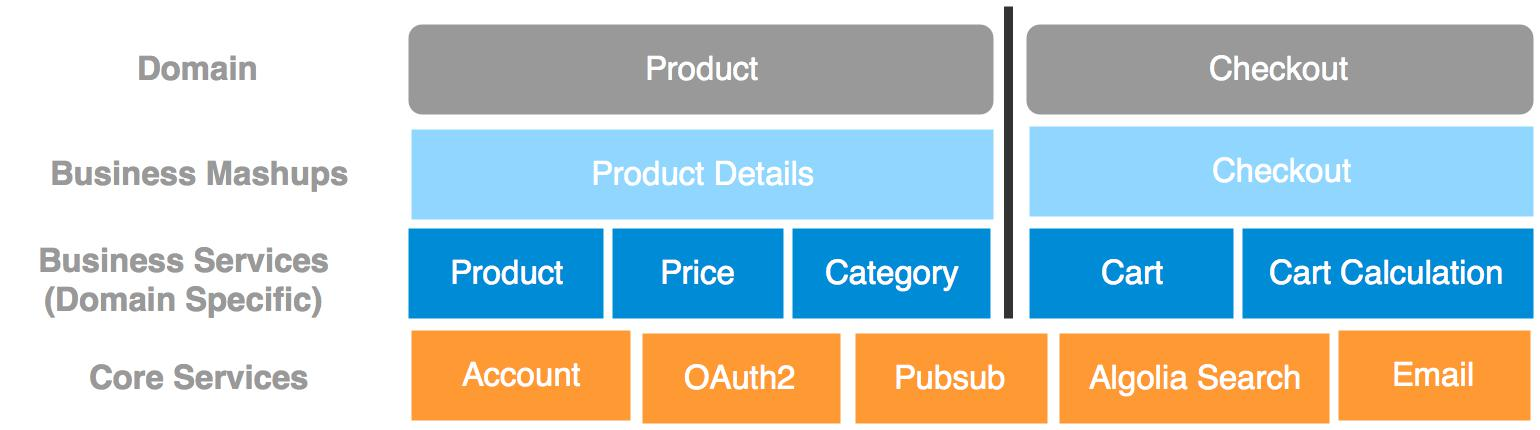
\includegraphics[width=0.8\textwidth]{figures/hybris_architecture_four}
\caption{Microservices Layers}
\label{fig:hybris_architecture/interview/microservices-layers}
\end{center}
\end{figure}
\\
\textbf{\underline{Step 4:}}
\\
The same process from steps 1-3 are applied to remaining sub-domains listed in Table \ref{tab:hybris_architecture/example_scenario/sub-domains-in-YaaS}. The Table \ref{tab:hybris_architecture/example_scenario/service_list_in_sub_domains} shows a list of services discovered in each sub-domains within the commerce domain. For example, 'Tax' and 'Tax Avalara' are microservices under 'Tax' sub-domain. Similarly, 'Order' and 'Order Details' are microservices related to 'Order' subdomain.
\begin{table}[H]
  \centering
  \begin{adjustbox}{max width=\textwidth}
  \begin{tabular}{*{14}{|c}|}%%{|c|c|}
  \hline
  \textbf{Sub-domain}  & \textbf{Microservice} & \textbf{Description}\\
  \hline
  \hline
    \multirow{3}{*}{Checkout}         & checkout          & handles the orchestration logic for checkout\\ 
   & cart          & handles cart inventory\\ 
   & Cart Calculation          & calculates net value of cart considering various constraints such as tax, discount etc.\\
   \hline \hline
   \multirow{4}{*}{Product}         & Product          & manages product inventory\\ 
   & Product Details          & provides mashup of product, price and category\\ 
   & Category          & manages category of products\\
   & Price         & manage price for products\\
   \hline
   \hline
   \multirow{2}{*}{Order}         & Order          & handles order management\\ 
   & Order Details          & provide mashup of orders and products\\ 
   \hline \hline
   \multirow{2}{*}{Site}         & Site          & handles site configuration\\ 
   & Shipping          & handles shipping configuration for site\\ 
   \hline \hline
   \multirow{2}{*}{Tax}         & Tax          & handles tax configuration\\ 
   & Tax Avalara          & handles tax calculation using Avalara\\ 
   \hline \hline
   Customer         & Customer    & deals with customer inventory\\ \hline \hline
   Coupon           & Coupon    & deals with coupon management \\ \hline \hline
   Payment  & Payment Stripe          & handles payment for oders using Stripe\\ \hline
   \hline
   \end{tabular}
\end{adjustbox}
  \caption{Services in \acrshort{YaaS} Commerce domain}
  \label{tab:hybris_architecture/example_scenario/service_list_in_sub_domains}
\end{table}
Including all the microservices in core, supporting and generic sub-domains for only commerce domain, the resulting architecture is as shown in Figure \ref{fig:hybris_architecture/interview/microservices_layers_commerce_domain}. At the bottom are various generic microservices such as Pubsub, Document etc. They are utilized by various business microservices such as Customer, Coupon etc. On the top are various mashup microservices such as Checkout, Order-Details and they utilize various business microservices and core microservices underneath.
\begin{figure}[H]
\begin{center}
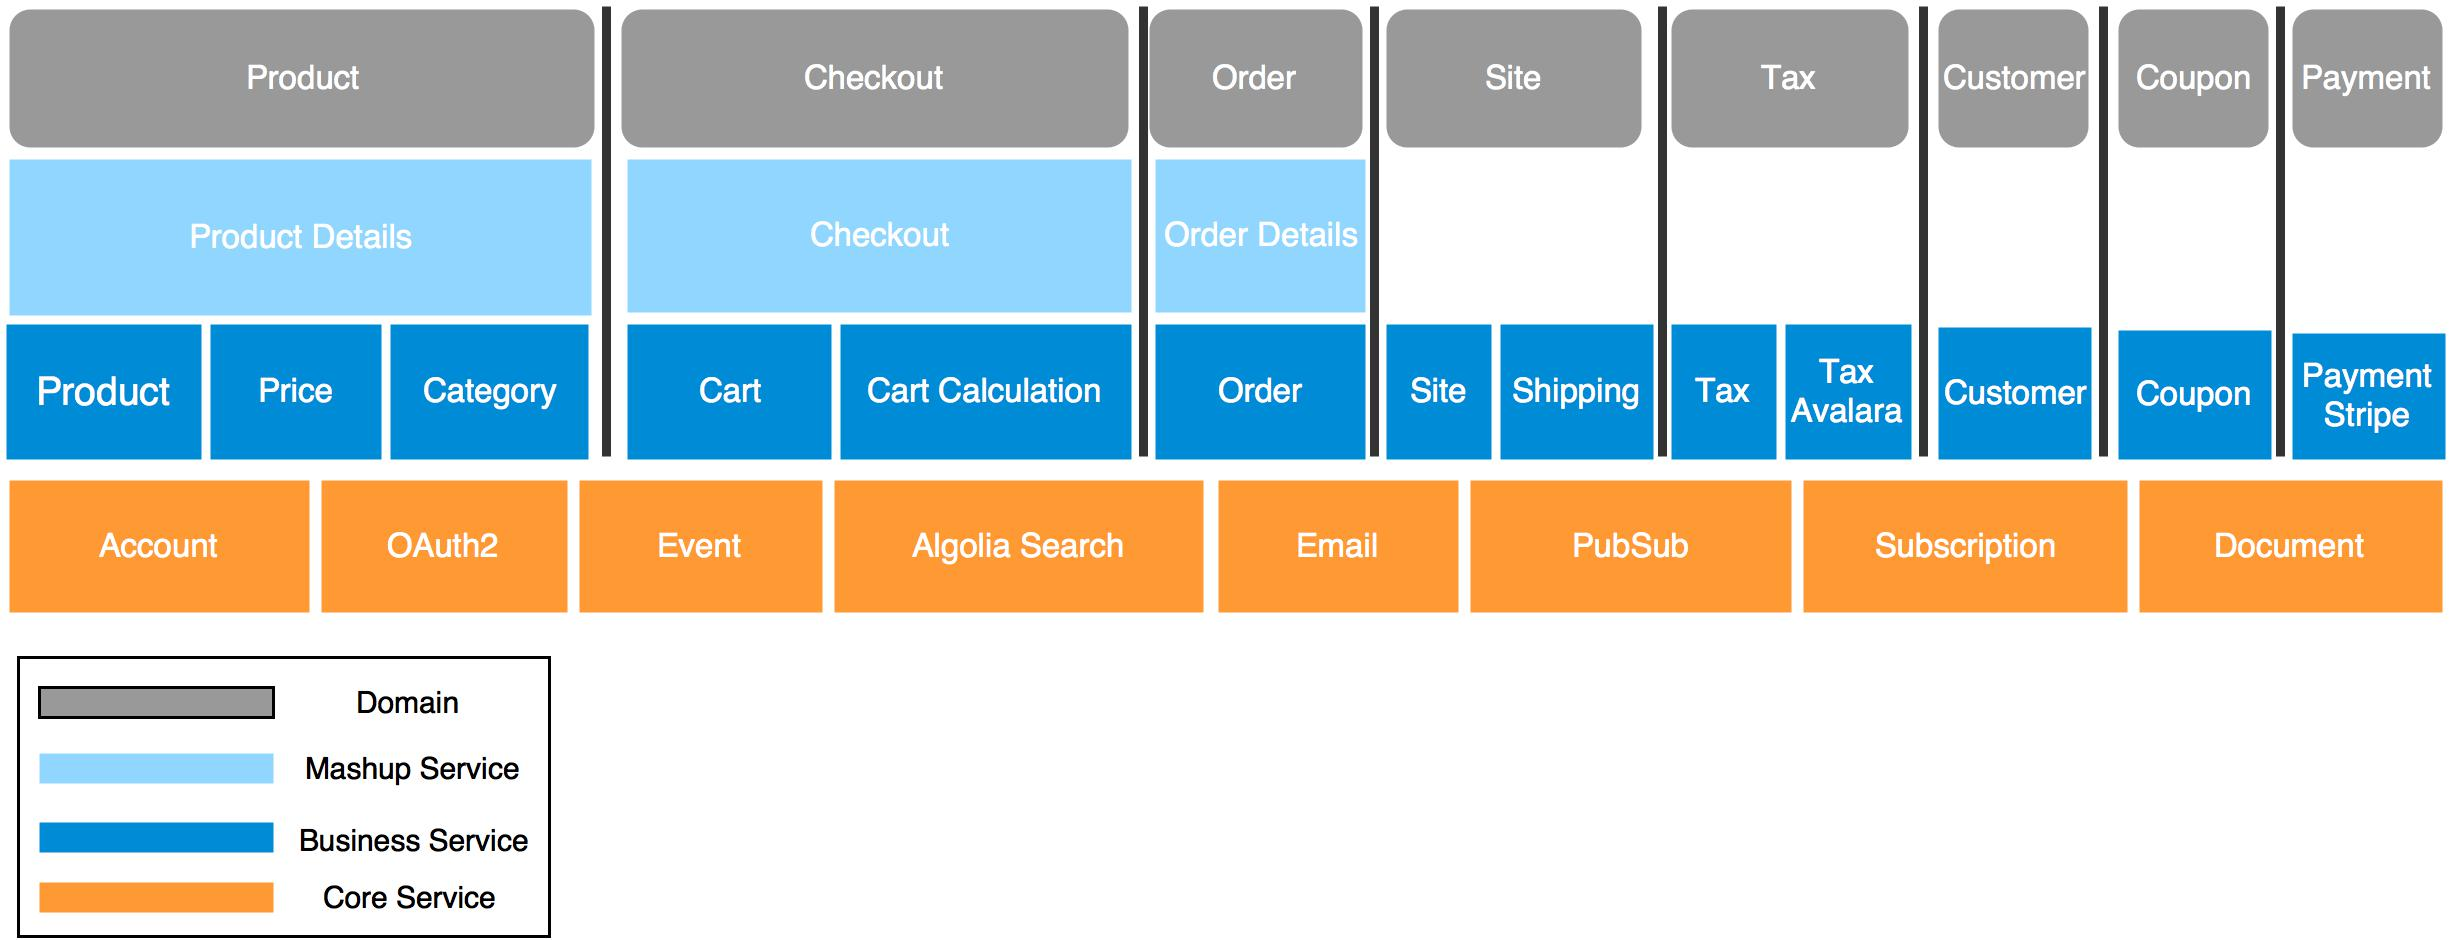
\includegraphics[width=0.9\textwidth]{figures/hybris_architecture_six}
\caption{Microservices Layers For Commerce Domain}
\label{fig:hybris_architecture/interview/microservices_layers_commerce_domain}
\end{center}
\end{figure}

\section{Deployment Workflow}\label{section:hybris_architecture/deployment_workflow}
Another major aspect apart from modeling microservices is continuous deployment. One of the major goals of implementing microservices architecture is agility. Agility can only be maintained when any small change in each microservice can be deployed into production smoothly without affecting other microservices.\\

\subsection{SourceCode Management}\label{section:hybris_architecture/deployment_workflow/sourcecode_management}
\begin{figure}[H]
\begin{center}
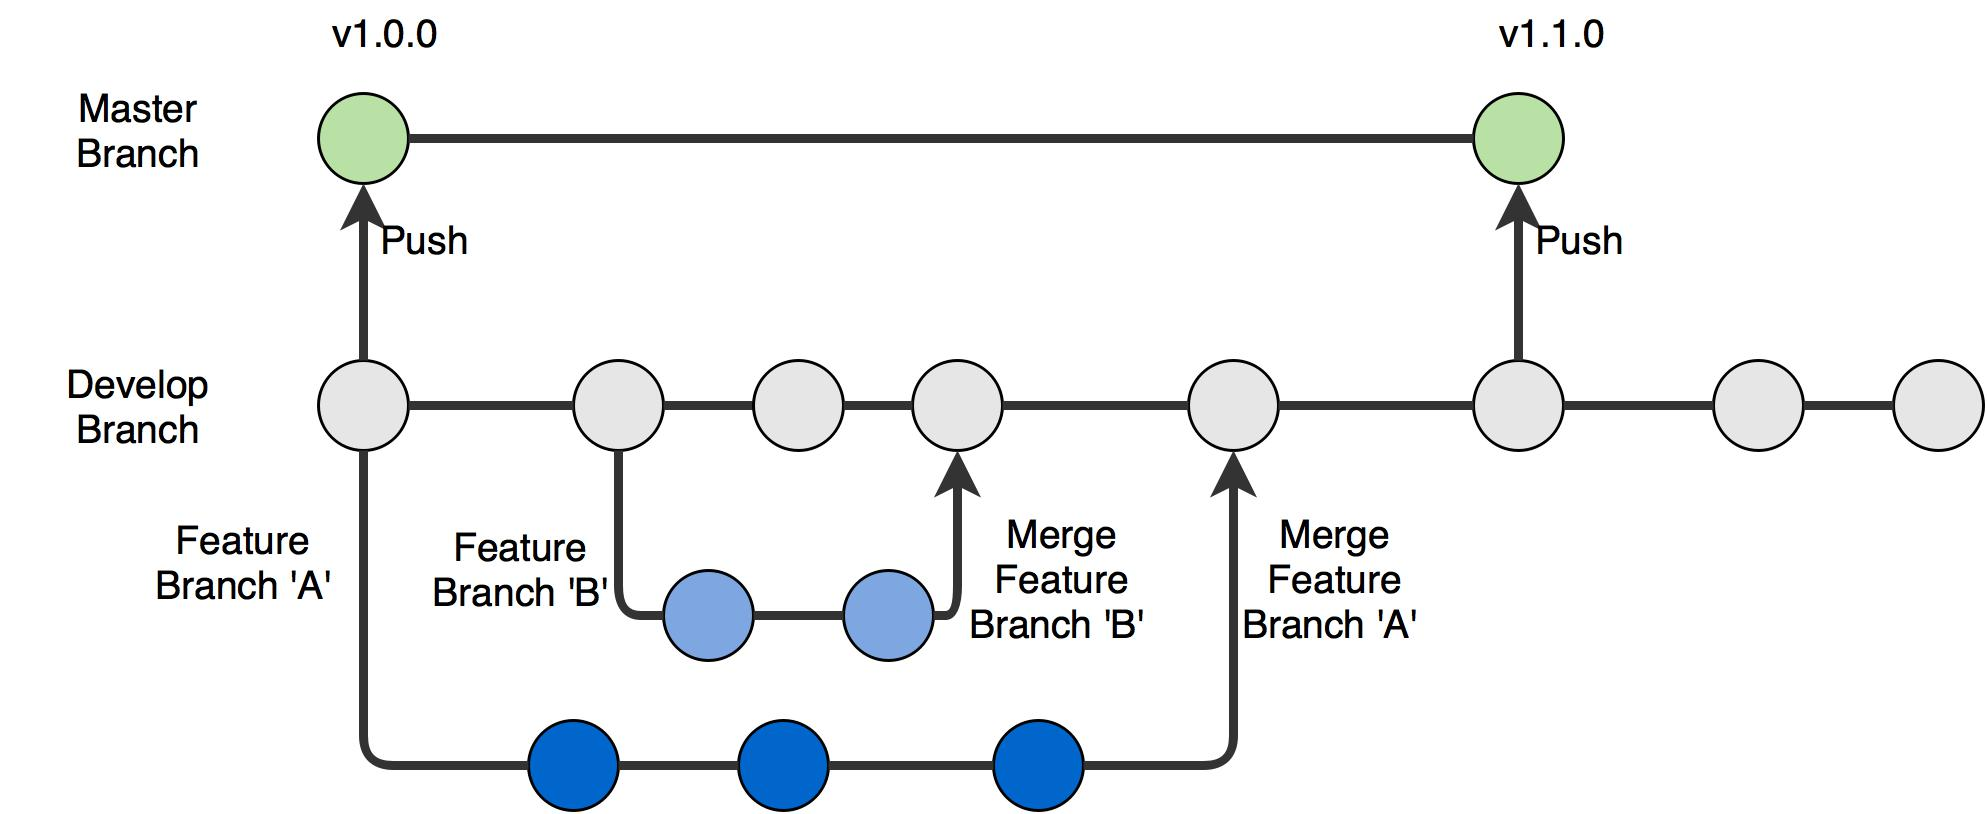
\includegraphics[width=0.9\textwidth]{figures/hybris_architecture_sourcecode_magement}
\caption{Sourcecode Management at SAP Hybris}
\label{fig:hybris_architecture/interview/sourcecode_management_at_hybris}
\end{center}
\end{figure}

The sourcecode files for each microservices are maintained in BitBucket version control system. The files are managed using Git. In order to support continuous deployment and efficient collaboration among the developers working in the same microservice, various branches are maintained within each repository. The major branch is called "Master" branch, which is used only for continuous deployment in production. Another branch is "Develop" branch and is used by developers to add changes continuously. It is used to create development version of the microservice and undergoes various level of tests. When sufficient features are ready and verified in "Develop" branch, they are merged into "Master" branch and realeased from "Master" branch. In this way, "Master" branch has always unbroken production ready sourcecode.
\\
For adding any major changes or features in the microservices, a new "Feature" branch is created from "Develop" branch and undergoes various levels of testing before it is merged with "Develop" branch. In this way, development and verification of any change can happen independently.

\subsection{Continuous Deployment}\label{section:hybris_architecture/deployment_workflow/continuous_Deployment}
In Section \ref{section:hybris_architecture/deployment_workflow/sourcecode_management}, the concept of maintaining feature branches are discussed. In this section, the process of deploying the changes of feature branch to the production is discussed.\\
The Figure \ref{fig:hybris_architecture/interview/continuous_deployment_flow} shows the complete deployment flow for a microservice. Firstly, a developer "A" pushes his/her local changes to the remote "Feature" branch at BitBucket. The changes triggers Teamcity "Build" phase where the changes are first compiled and then a series of unit tests run against the newly built application which is again followed by a series of integration tests.\\
If the tests are successful, the developer will create a pull request in BitBucket, representing a request to merge his/her changes to "Develop" branch. Developer "B" from the same team will then review his/her changes and provides comments on BitBucket interface. After the changes are made and developer "B" is satisfied, he/she approves the pull request.\\
The developer "A" or "B" can merge the feature branch into develop branch. This again triggers "Build" phase in Teamcity. In "Build" phase, the develop branch gets compiled, followed by unit tests and integration tests. If the tests are successful, then "Deployment" phase is triggered when code is deployed to "Stage" environment and a group of smoke tests run to verify the deployment. Now, project owner or quality assurance team can access the microservice from stage and perform user acceptance tests. If there are any feedbacks or changes to be made, it will follow the same process from the beginning.\\
Now, when there are sufficient features and it is time for release, the "Develop" branch is merged to "Master" branch. The merge will again trigger "Build" phase in Teamcity. After successful tests, the "Master" branch is first deployed into "Stage" environment, where a series of smoke tests runs. After the deployment is successful without any error, the "Master" branch is deployed into "Production" environment, where various smoke tests run again to re-assure the deployment.
\begin{figure}[H]
\begin{center}
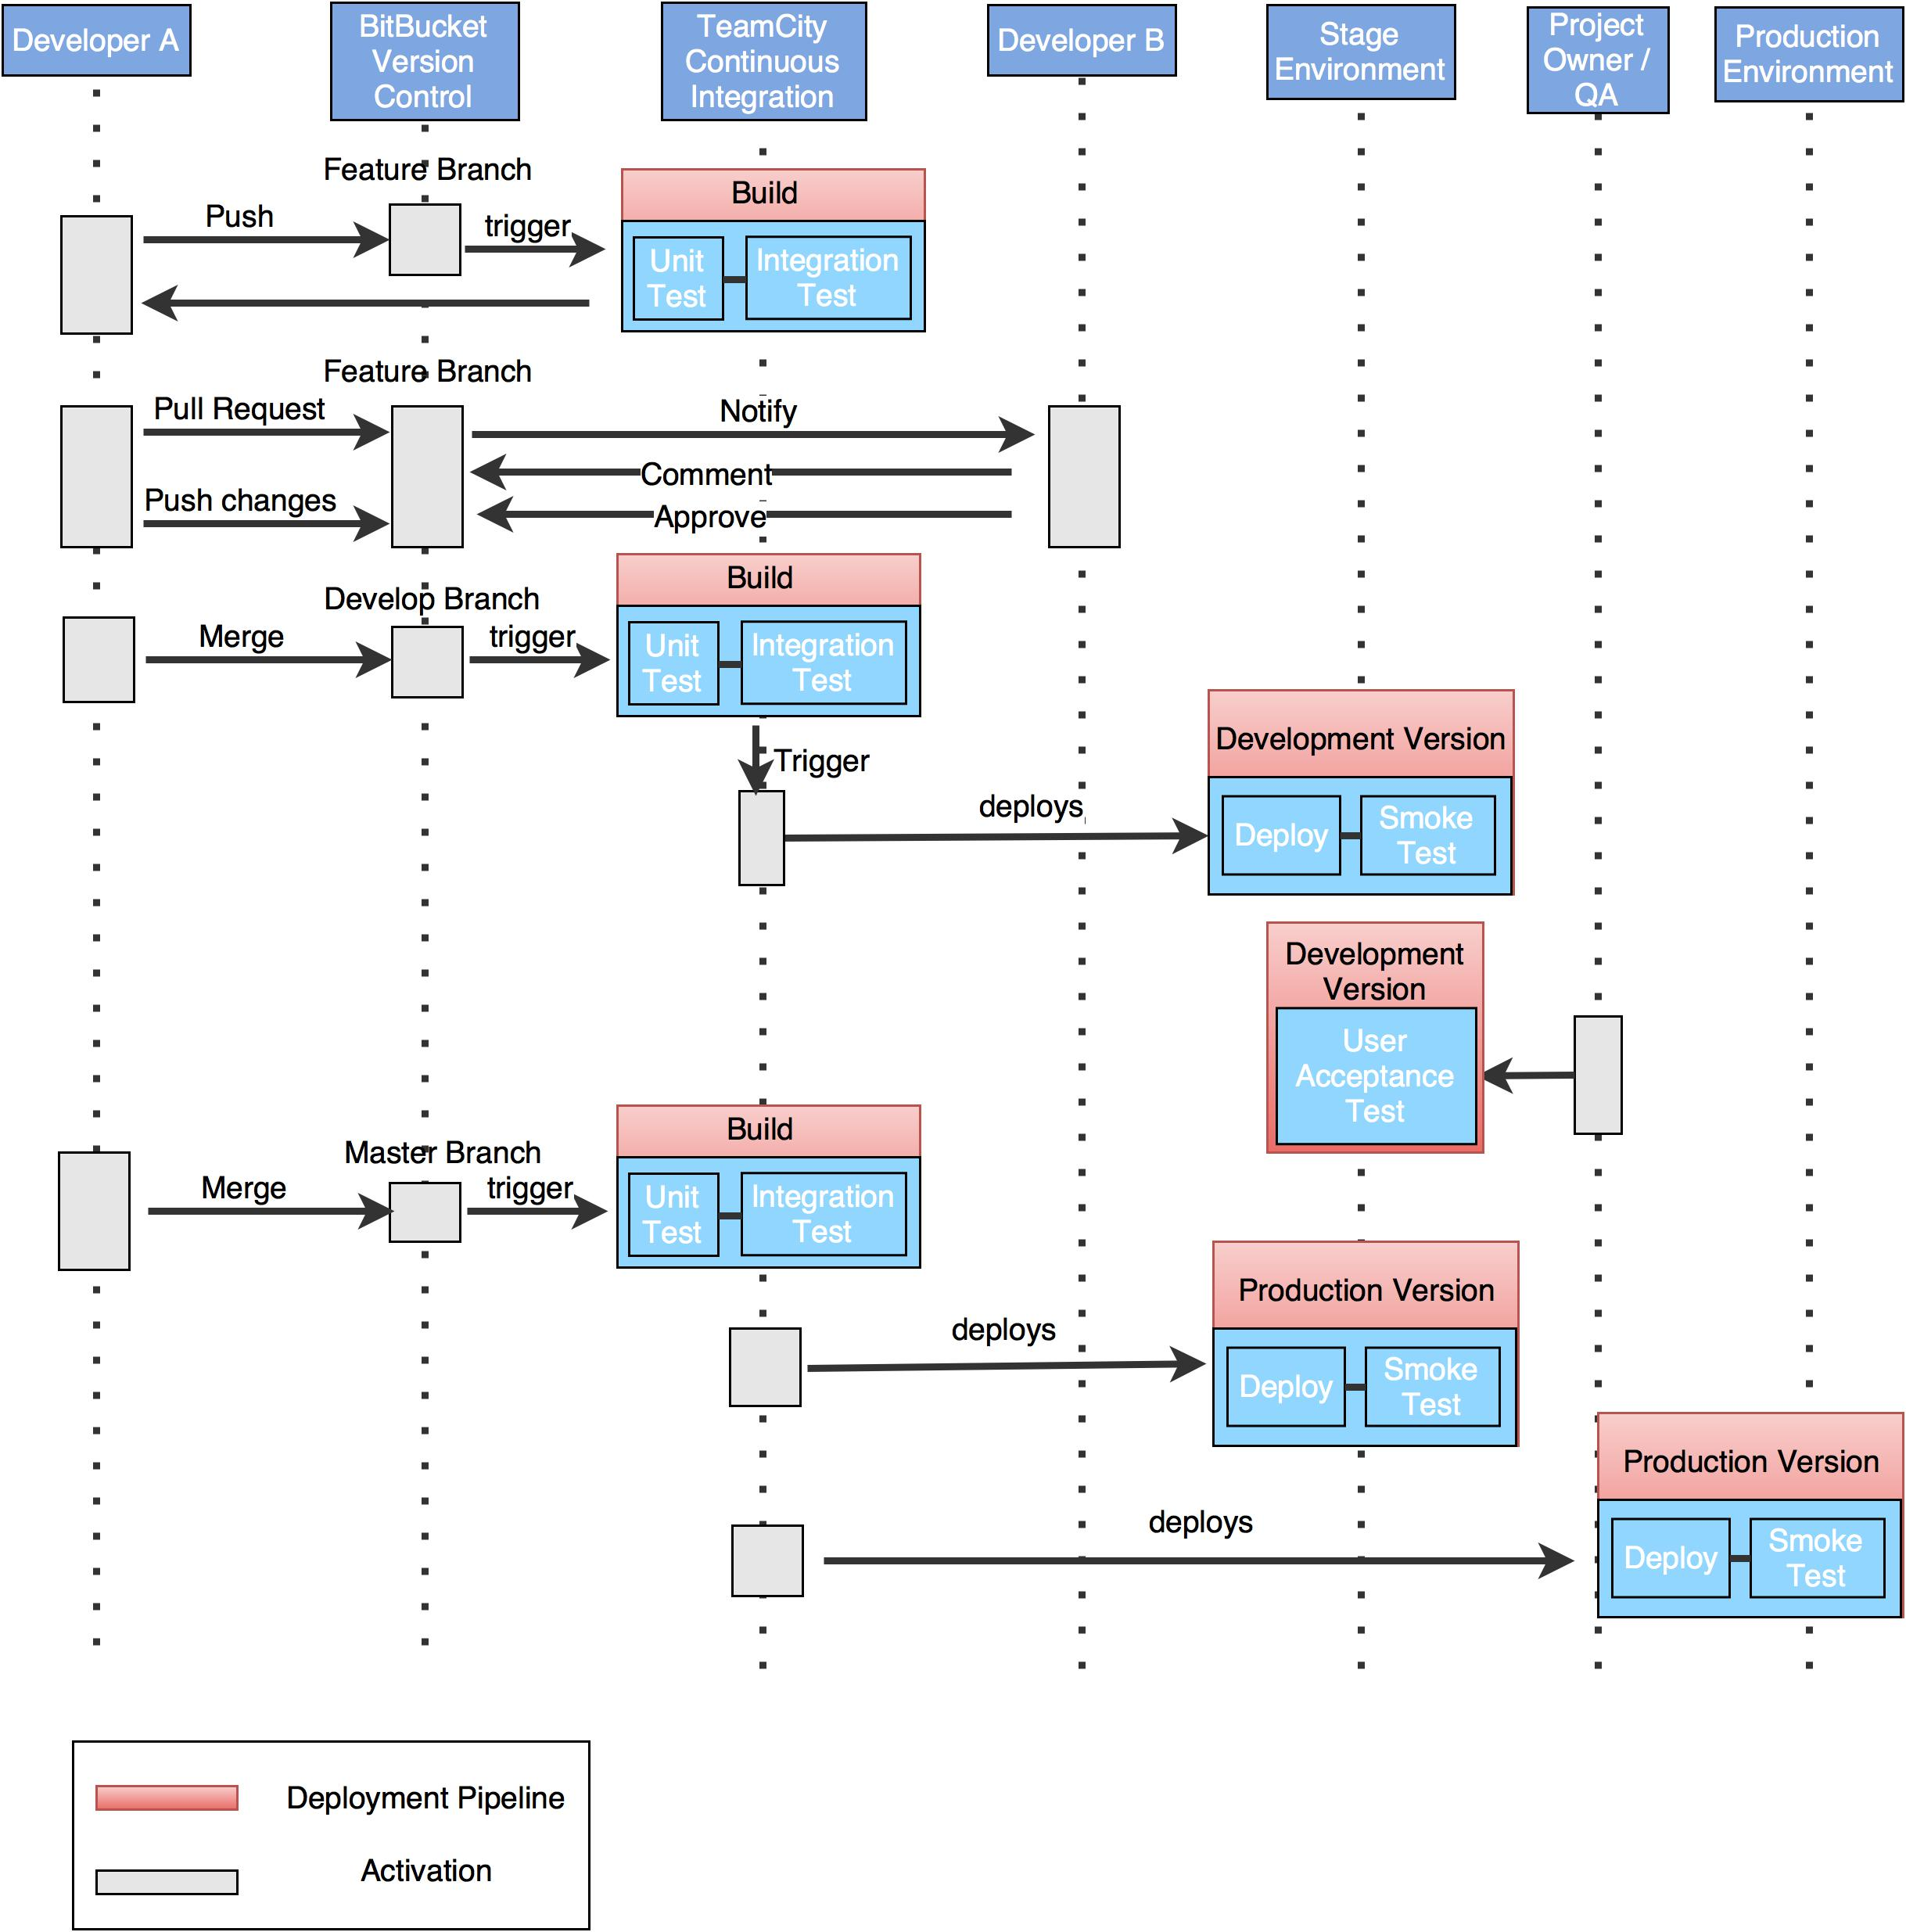
\includegraphics[width=0.9\textwidth]{figures/hybris_architecture_continuous_deployment_flow}
\caption{Continuous Deployment at SAP Hybris}
\label{fig:hybris_architecture/interview/continuous_deployment_flow}
\end{center}
\end{figure}

The deployment is performed using cloud foundry which consists of \acrshort{AWS} cloud underneath.
The Figure \ref{fig:hybris_architecture/interview/microservices_layers_commerce_domain} uncovers only microservices at the backend related to commerce domain. The complete architecture covering other domains such as Marketing etc and all layers including User-Interface, \acrshort{PaaS} is shown by Figure \ref{fig:hybris_architecture/interview/hybris-architecture}. Apart from Commerce domain, there are various other domains such as Marketing, Sales etc. On each domain, same process as discussed in the Case Study \ref{section:hybris_architecture/example_scenario} is followed to identify various microservices. For example, in 'Marketing' domain, there are microservices such as 'Loyalty', Loyalty Mashup' services.
\\
\begin{figure}[H]
\begin{center}
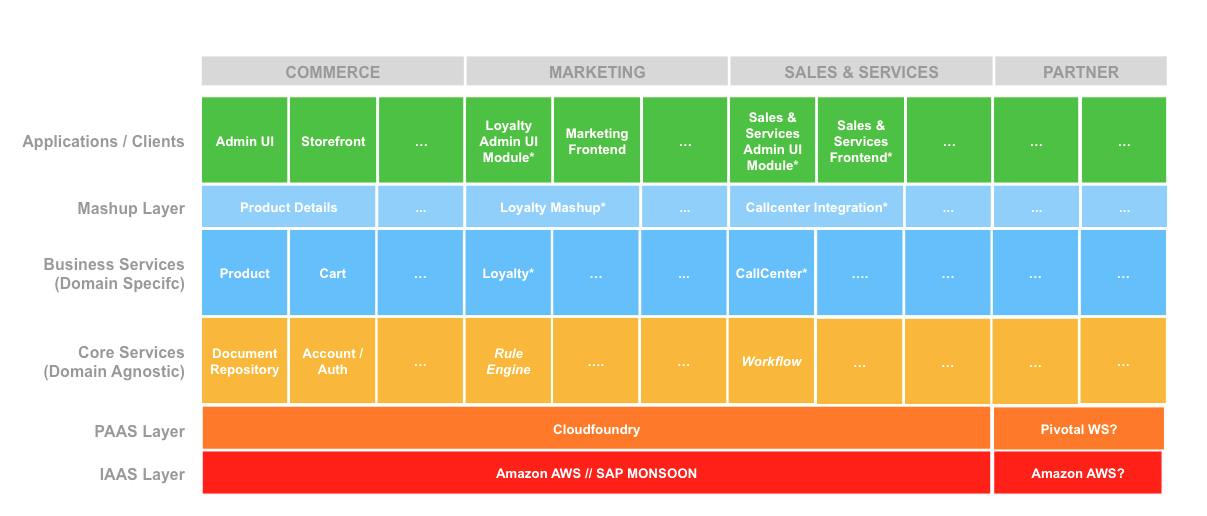
\includegraphics[width=0.9\textwidth]{figures/hybris-architecture-five}
\caption{SAP Hybris Architecture}
\label{fig:hybris_architecture/interview/hybris-architecture}
\end{center}
\end{figure}

\section{Summary}\label{section: hybris_architecture/problem_statement}
In this chapter, the modeling approach used in SAP Hybris is discussed. Again, the continuous deployment process for each microservice is presented. This adds value to the findings made regarding modeling process from literature review. Now, as stated in Section \ref{section:context/approach}, the constraints or challenges are one of the drivers for defining guidelines. So, the next step is to research about various challenges when implementing microservices and find the techniques to tackle them. While looking into that, it can also be interesting to find out how these challenges are being handled at SAP Hybris.












